% Created 2015-02-20 Пт 06:18
\documentclass[presentation]{beamer}
\useoutertheme[subsection=true]{miniframes}%{miniframes}

%%% Packages.

\usepackage[utf8]{inputenc}
\usepackage[T1]{fontenc}
\usepackage{fixltx2e}
\usepackage{graphicx}
\usepackage{longtable}
\usepackage{float}
\usepackage{wrapfig}
\usepackage{rotating}
\usepackage[normalem]{ulem}
\usepackage{amsmath, amssymb}
\usepackage{textcomp}
\usepackage{marvosym}
\usepackage{wasysym}
\usepackage{hyperref}
\tolerance=1000
\usepackage[english, russian]{babel}
\usepackage[labelformat=empty]{caption}
\usepackage{subcaption}
\usepackage{color}
\let\Cross\relax
\let\Square\relax
\usepackage{bbding}
\usepackage{fancyvrb}
\usepackage{textpos}

% Орнаменты
\usepackage{fourier-orns}
\usepackage{pgfornament}


%%%

\setbeamertemplate{headline}{}

\graphicspath{{graphics/}}

\definecolor{old_paper}{RGB}{242, 227, 208}
\definecolor{old_title_font}{RGB}{238, 206, 147}
\setbeamercolor{background canvas}{bg=old_paper}

\setbeamercolor{titlelike}{fg=old_title_font}
\setbeamercolor{title}{fg=old_title_font}
\setbeamercolor{frametitle}{fg=old_title_font}

\addtobeamertemplate{title page}{
  \begin{textblock*}{\paperwidth}(-39pt, -52pt)
  
\includegraphics[width=1.1\paperwidth, height=1.1\paperheight]{popularsciencemo09newy_0001}
  \end{textblock*}
}

\setbeamercolor{author}{fg=old_title_font}
\setbeamercolor{date}{fg=old_title_font}

\setbeamertemplate{frametitle}[default][center]
\addtobeamertemplate{frametitle}{
  \begin{textblock*}{\paperwidth}(-30pt, -30pt)
    
\includegraphics[width=1.1\paperwidth, height=2cm]{title-bg}
  \end{textblock*}
}

\setbeamertemplate{background}{
  
\includegraphics[width=\paperwidth,height=\paperheight,keepaspectratio]{frame-bg}
}

\useinnertheme{circles}
\setbeamertemplate{itemize item}{
  \color{black}
  \scriptsize\raise1.25pt\hbox{\donotcoloroutermaths$\bullet$}
}

\setbeamercolor{item projected}{bg=black}

\hypersetup{colorlinks = true}

\hypersetup{linkcolor=black}
\hypersetup{linkbordercolor=black}
\hypersetup{urlcolor=black}

\beamertemplatenavigationsymbolsempty


%%% Macros.

\newcommand{\RaisedLeftHand}{%
  \raisebox{-.50em}{\Large\HandLeft}
}

\newcommand{\RaisedRightHand}{%
  \raisebox{-.50em}{\Large\HandRight}
}

\newcommand{\EndOfSectionOrnament}{
  \begin{center}
    \pgfornament[width=0.5\textwidth]{88}
    \end{center}
}


%%% Title.

\author{АРТЁМ ПОПЦОВ}
\date{2017-02-12}

\title{\decofourleft\hspace{.30em} КРИПТОГРАФИЯ \hspace{.30em}\decofourright}
\subtitle{КОТОРАЯ ПРОСТО РАБОТАЕТ}

\begin{document}

\maketitle


%%% TOC.

\begin{frame}{\sc{Содержание.}}
  \setcounter{tocdepth}{1}
  \tableofcontents
\end{frame}


%%%

\section{\sc{Постановка задачи.}}

\begin{frame}{\sc{Постановка задачи.}}
  \begin{figure}[htb]
    \centering
    
\includegraphics[width=1.0\textwidth]{network-1}
  \end{figure}
  \RaisedRightHand Необходимо обеспечить три параметра:
  \begin{itemize}
  \item Конфиденциальность
  \item Целостность
  \item Аутентификацию
  \end{itemize}
\end{frame}

\begin{frame}{\sc{Реальность.}}
  \begin{figure}[htb]
    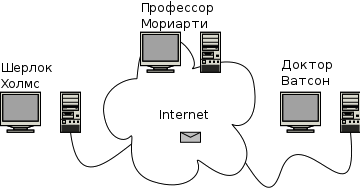
\includegraphics[width=1.0\textwidth]{network-2}
    \llap{
      \put(-250,100){
        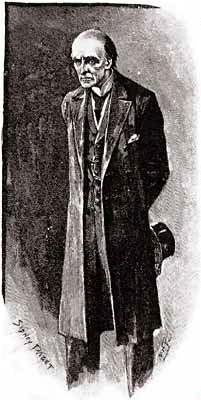
\includegraphics[height=0.4\textheight]{Pd_Moriarty_by_Sidney_Paget}
      }
    }
  \end{figure}
\end{frame}


%%%

\section{\sc{Выбор инструмента.}}

\begin{frame}{\sc{Выбор инструмента.}}
  \begin{quote}
    ``Криптография -- единственный набор инструментов для обеспечения
    безопасности в интернете, который у нас есть.  Мы открываем наш
    ящик с инструментами и всё, что мы имеем -- криптомолоток.'' -- Ян Голдберг
\end{quote}

  \bigskip

  \begin{columns}
    \begin{column}{0.6\textwidth}

Характеристики хорошего инструмента:
\begin{itemize}
\item Удобство использования (англ. \textit{usability})
\item Доступность (англ. \textit{deployability})
\item Эффективность (англ. \textit{effectiveness})
\item Надёжность (англ. \textit{robustness})
\end{itemize}
    \end{column}
    \begin{column}{0.4\textwidth}
      \begin{figure}[htb]
        \centering
        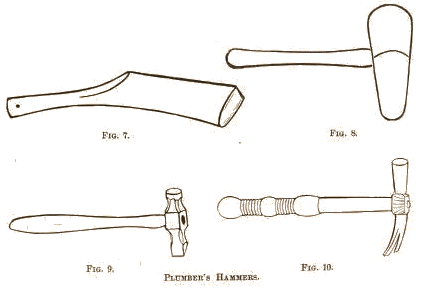
\includegraphics[width=1.0\textwidth]{popularsciencemo09newy_0033}
      \end{figure}
      \end{column}
  \end{columns}
\end{frame}

\begin{frame}{\sc{Удобство использования.}}
  \begin{columns}
    \begin{column}{0.6\textwidth}
      \RaisedRightHand Инструмент должен быть удобен для
      использования.

      \bigskip

      \begin{itemize}
      \item Необходим понятный интерфейс, упрощающий корректное
        использование инструмента.
        % Некорректное использование криптографии инструмента может
        % привести к иллюзии защищённости, что гораздо хуже, чем если бы
        % инструмент не был использован в принципе.
        % См. также "Принцип наименьшего удивления."
      \item В идеале, инструмент должен оказывать минимальное влияние на
        рабочий процесс пользователя.
      \end{itemize}
    \end{column}
    \begin{column}{0.4\textwidth}
      \begin{figure}[htb]
        \centering
        
\includegraphics[height=.8\textheight]{hammer-use-0}
      \end{figure}
      \end{column}
  \end{columns}

\end{frame}

\begin{frame}{\sc{Доступность.}}
  \RaisedRightHand Инструмент должен
  предъявлять разумные требования, иначе его никто не будет
  использовать.

  \bigskip

  \begin{itemize}
  \item Необходима интеграция с существующим рабочим окружением
    пользователя, а не наоборот.
  \end{itemize}

  \begin{figure}[htb]
    \centering
    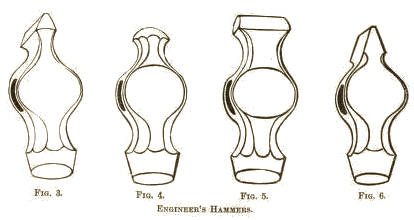
\includegraphics[height=.4\textheight]{hammer-01}
  \end{figure}
\end{frame}

\begin{frame}{\sc{Эффективность.}}
  \RaisedRightHand Инструмент должен обеспечивать характеристики,
  которые были "по гарантии".\newline\newline

  \bigskip

  \begin{columns}
    \begin{column}{0.6\textwidth}
      \begin{itemize}
      \item Сообщество должно иметь возможность провести независимый аудит
        инструмента.
      \item Следовательно, исходный код инструмента, документация и
        описание протоколов должны быть доступны сообществу (желательно,
        под свободной лицензией.)
      \end{itemize}
    \end{column}
    \begin{column}{0.4\textwidth}
      \begin{figure}[]
        \centering
        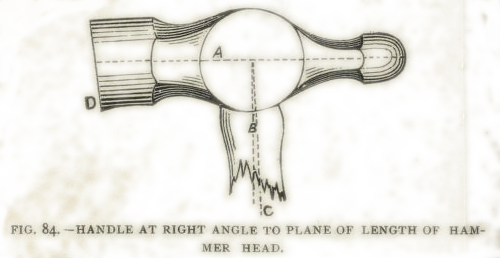
\includegraphics[width=1.1\textwidth]{hammer-00}
      \end{figure}
    \end{column}
  \end{columns}
\end{frame}

\begin{frame}{\sc{Надёжность.}}
  \raisebox{-.30em}{\Large\HandRight}\hspace{.25em} Если ``что-то
  пошло не так'', то инструмент должен сделать всё возможное, чтобы
  уменьшить урон.

  \bigskip

  \begin{quote}
    ``[...] a general principle of robustness: be conservative in what
    you do, be liberal in what you accept from others.'' -- Jon Postel
  \end{quote}

  \bigskip

  (Общий принцип надёжности Джона Постела: будьте консервативны в том,
  что делаете, и либеральны в том, что получаете от других.)

  \EndOfSectionOrnament
\end{frame}


%%%

\section{\sc{Доступные  Инструменты.}}

\begin{frame}{\sc{Доступные инструменты.}}
  \begin{itemize}
  \item GNU Privacy Guard (GnuPG)
  \item Off-The-Record Messaging (OTR)
  \end{itemize}
  \begin{figure}[htb]
    \centering
    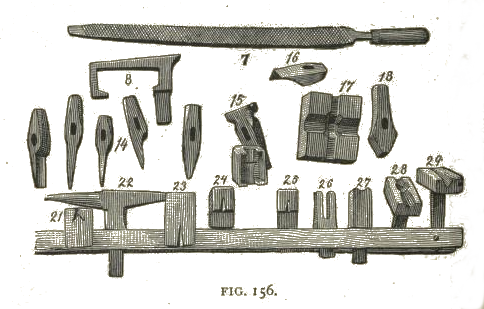
\includegraphics[height=0.6\textheight]{hammer-02.png}
  \end{figure}
\end{frame}


%%%

\section{\sc{GNU Privacy Guard.}}

\begin{frame}{\sc{GNU Privacy Guard.}}
  \RaisedRightHand GNU Privacy Guard
  (GnuPG) -- свободная программа шифрования информации и создания
  электронных цифровых подписей (ЭЦП).

  \begin{itemize}
  \item GnuPG относительно удобен в использовании, есть дружественные
    графические интерфейсы.
  \item Программа доступна на большинстве платформ и интегрируется с
    рабочим окружением пользователя.
  \end{itemize}

  Задачи, решаемые с помощью GnuPG:
  \begin{itemize}
  \item Электронная подпись данных
  \item Шифрование данных
  \end{itemize}
\end{frame}

\begin{frame}[fragile]{\sc{Установка GnuPG.}}
  На большинстве дистрибутивов GNU/Linux GnuPG можно поставить из
  репозитория.  Пример для Ubuntu GNU/Linux:
\begin{Verbatim}[commandchars=\\\[\]]
\$ sudo apt-get install gnupg gnupg-agent
\end{Verbatim}
\vspace{5 mm}

На Microsoft Windows можно воспользоваться \textbf{Gpg4win}
(\url{https://www.gpg4win.org/}).\newline

\RaisedRightHand Руководство от Electronic Frontier Foundation:
\begin{itemize}
\item \url{https://ssd.eff.org/ru}
\end{itemize}
\RaisedRightHand ``Самозащита электронной почты'' от Free Software
Foundation:
\begin{itemize}
\item \url{https://emailselfdefense.fsf.org/ru/}
\end{itemize}
\end{frame}


%%%

\subsection{Криптография с открытым ключом.}

\begin{frame}{\sc{Криптография с открытым ключом -- 1.}}
  \begin{columns}
    \begin{column}{0.7\textwidth}
      \raisebox{-.30em}{\Large\HandRight}\hspace{.25em} Криптография с
      открытым ключом (или \textit{ассиметричная криптография}) -- система
      шифрования и/или электронной подписи, при которой используется пара
      открытый ключ-закрытый ключ, и открытый ключ передаётся по
      незащищённому каналу.
    \end{column}
    \begin{column}{0.3\textwidth}
      \begin{figure}[htb]
        \centering
        
\includegraphics[height=0.8\textheight]{keys}
      \end{figure}
    \end{column}
  \end{columns}
\end{frame}

\begin{frame}{\sc{Криптография с открытым ключом -- 2.}}
  \begin{figure}[htb]
    \centering
    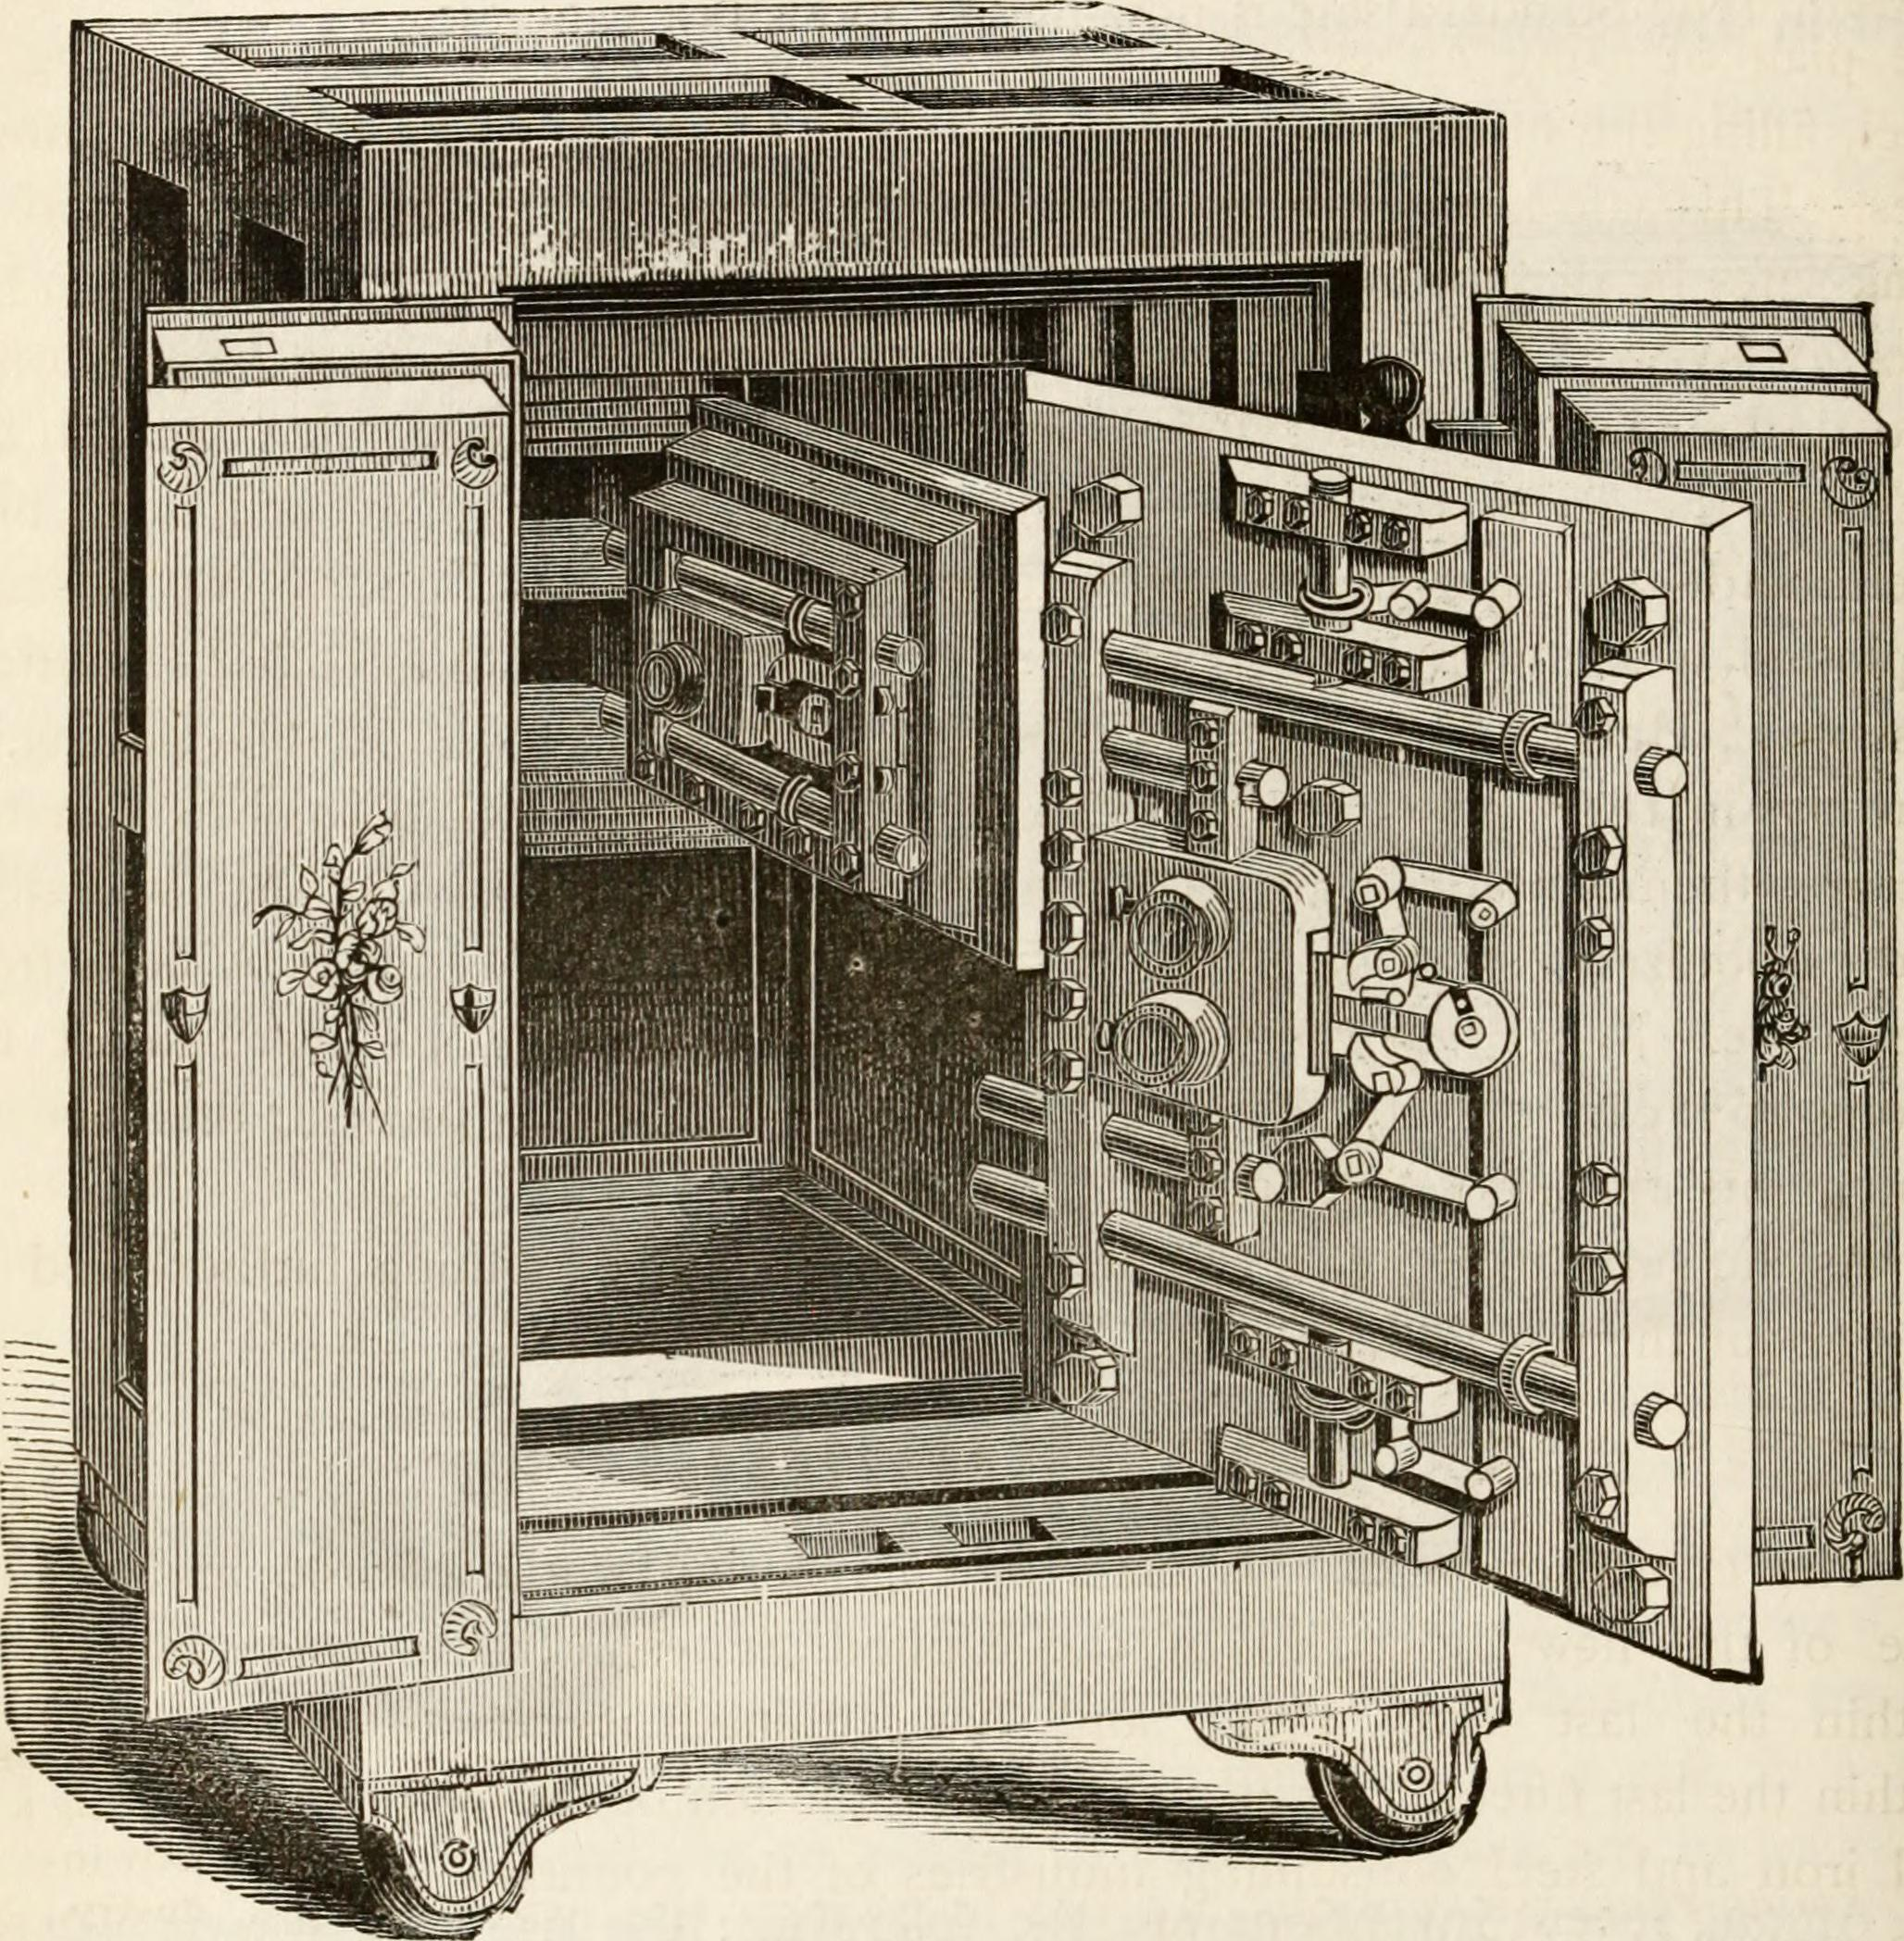
\includegraphics[height=0.6\textheight]{safe-00}
  \end{figure}
\end{frame}


%%%

\subsection{Создание пары ключей}

\begin{frame}[fragile]{\sc{Создание пары ключей -- 1.}}
  Пара ``закрытый ключ -- публичный ключ'' может быть создана
  следующей командой:
\begin{verbatim}
$ gpg --gen-key
\end{verbatim}
  При создании ключа необходимо:
  \begin{enumerate}
  \item Выбрать тип ключа:
    \small
\begin{Verbatim}[commandchars=\\\[\]]
Please select what kind of key you want:
   (1) RSA and RSA (default)
   (2) DSA and Elgamal
   (3) DSA (sign only)
   (4) RSA (sign only)
Your selection? 1 [\RaisedLeftHand]
\end{Verbatim}
\normalsize
    \end{enumerate}
\end{frame}

\begin{frame}[fragile]{\sc{Создание пары ключей -- 2.}}
  \begin{enumerate}
    \setcounter{enumi}{1}
  \item Выбрать длину ключа:
    \small
\begin{Verbatim}[commandchars=\\\[\]]
RSA keys may be between 1024 and 4096 bits long.
What keysize do you want? (2048) 2048 [\RaisedLeftHand]
Requested keysize is 2048 bits
\end{Verbatim}
\normalsize
\item Выбрать ``срок годности'' ключа:
  \small
\begin{Verbatim}[commandchars=\\\[\]]
Please specify how long the key should be valid.
         0 = key does not expire
      <n>  = key expires in n days
      <n>w = key expires in n weeks
      <n>m = key expires in n months
      <n>y = key expires in n years
Key is valid for? (0) 1y [\RaisedLeftHand]
Key does not expire at all
Is this correct? (y/N) y [\RaisedLeftHand]
\end{Verbatim}
\normalsize
    \end{enumerate}
\end{frame}

\begin{frame}[fragile]{\sc{Создание пары ключей -- 3.}}
  \begin{enumerate}
    \setcounter{enumi}{3}
  \item Указать реальное имя владельца ключа:
    \small
\begin{Verbatim}[commandchars=\\\[\]]
Real name: Vasiliy I. Pupkin [\RaisedLeftHand]
\end{Verbatim}
  \item Указать адрес электронной почты владельца:
\begin{Verbatim}[commandchars=\\\[\]]
Email address: vip@example.ru [\RaisedLeftHand]
\end{Verbatim}

  \item (Опционально) указать комментарий к ключу.
\item Проверить указанную информацию и подтвердить её:
  \small
  \begin{Verbatim}[commandchars=\\\[\]]
You selected this USER-ID:
    "Vasiliy I. Pupkin <vip@example.ru>"

Change (N)ame, (C)omment, (E)mail
  or (O)kay/(Q)uit? O [\RaisedLeftHand]
  \end{Verbatim}
  \normalsize
\item Задать пароль для доступа к закрытому ключу.
\item ``Пошуметь'' для генерации достаточного количества энтропии.
    \end{enumerate}

\end{frame}

\begin{frame}[fragile]{\sc{Создание пары ключей -- 4.}}
  Результат:
  \begin{Verbatim}[commandchars=\\\[\]]
\$ gpg --list-secret-keys
/home/vip/.gnupg/secring.gpg
----------------------------
sec   2048R/F4A78166 2016-08-29
uid                  Vasiliy I. Pupkin <vip@example.ru>
ssb   2048R/BAED1502 2016-08-29
  \end{Verbatim}
  \EndOfSectionOrnament
\end{frame}


%%%

\subsection{Сертификат отзыва ключа}

\begin{frame}[fragile]{\sc{Сертификат отзыва ключа.}}
  \raisebox{-.30em}{\Large\HandRight}\hspace{.25em} Сертификат отзыва
  ключа (англ. \emph{revocation certificate}) -- Сертификат, который,
  будучи опубликованным, говорит о том, что связанный с ним ключ более
  не должен использоваться.\newline

  \begin{itemize}
  \item Сертификат должен храниться в безопасном месте (например, в
    сейфе.)
  \item Сертификат должен быть создан сразу после генерации приватного
    ключа.\newline
  \end{itemize}
  
  Случаи, при которых необходимо отзывать ключ:
  \begin{itemize}
  \item Забыт (утерян) пароль к ключу.
  \item Ключ был скомпроментирован.
  \item Ключ более не действителен.
  \item \ldots{}
  \end{itemize}
\end{frame}

\begin{frame}[fragile]{\sc{Генерация сертификата отзыва ключа.}}
  \small
\begin{Verbatim}[commandchars=\\\[\]]
\$ gpg --output revoke.asc --gen-revoke F4A78166

sec  2048R/F4A78166 2016-08-29
  Vasiliy I. Pupkin <vip@example.ru>

Create a revocation certificate for this key? (y/N) y
Please select the reason for the revocation:
  0 = No reason specified
  1 = Key has been compromised
  2 = Key is superseded
  3 = Key is no longer used
  Q = Cancel
(Probably you want to select 1 here)
Your decision? 1 [\RaisedLeftHand]
\end{Verbatim}
\normalsize
\EndOfSectionOrnament
\end{frame}

\begin{frame}[fragile]{\sc{Отзыв ключа.}}
  \RaisedRightHand Вы не должны выполнять отзыв ключа без причины!

  \begin{itemize}
  \item Импортировать сертификат:
    \footnotesize
\begin{Verbatim}[commandchars=\\\[\]]
\$ gpg --import revoke.asc
gpg: key F4A78166: "Vasiliy I. Pupkin <vip@example.ru>"
     revocation certificate imported
gpg: Total number processed: 1
gpg:    new key revocations: 1
gpg: 3 marginal(s) needed, 1 complete(s) needed, PGP trust model
gpg: depth: 0  valid:   3  signed:   0
     trust: 0-, 0q, 0n, 0m, 0f, 3u
\end{Verbatim}
    \normalsize
  \item Загрузить обновлённый ключ на сервер:
    \footnotesize
\begin{Verbatim}[commandchars=\\\[\]]
\$ gpg --keyserver gpg.mit.edu --send-keys F4A78166
\end{Verbatim}
    \normalsize
  \end{itemize}
  \EndOfSectionOrnament
\end{frame}


%%%

\subsection{Электронная подпись.}

\begin{frame}[fragile]{\sc{Электронная подпись.}}
  Электронная подпись обеспечивает следующие свойства:
  \begin{itemize}
  \item \textbf{Целостность} -- гарантия отсутствия искажений данных с
    момента формирования подписи.
  \item \textbf{Авторство} -- принадлежность подписи владельцу ключа.
  \item \textbf{Неотказуемость} -- фиксирование невозможности отказа от
    авторства
  \end{itemize}

  \vspace{5 mm}

  Примеры практического применения электронных подписей:
  \begin{itemize}
  \item Подпись важных писем и документов.
  \item Подпись релизов пакетов в DVCS Git.
  \item Подпись дистрибутивов программ.
  \item \ldots{}
  \end{itemize}
\end{frame}

\begin{frame}[fragile]{\sc{Электронная подпись файлов.}}
  Подписать файл можно следующим образом:
\begin{verbatim}
$ touch important-file.txt
$ gpg --detach-sign important-file.txt
\end{verbatim}

  Электронная подпись будет сохранена файле
  \texttt{important-file.txt.sig}:
\begin{verbatim}
$ ls important-file*
important-file.txt important-file.txt.sig
\end{verbatim}

  Проверка подписи:
\begin{verbatim}
$ gpg --verify important-file.txt.sig
\end{verbatim}

  \EndOfSectionOrnament
\end{frame}


%%%

\subsection{Шифрование.}

\begin{frame}[fragile]{\sc{Шифрование.}}
  \begin{enumerate}
    
  \item \textbf{Ассиметричное} шифрование документа для доктора
    Ватсона с помощью его открытого ключа:
\begin{verbatim}
$ gpg --output doc.gpg --encrypt --recipient \
    dr.watson@example.ru doc
\end{verbatim}

  Расшифровка ранее зашифрованного документа с помощью приватного
  ключа доктора Ватсона:
\begin{verbatim}
$ gpg --output doc --decrypt doc.gpg
\end{verbatim}

\item Или можно использовать \textbf{симметричное} шифрование:
\begin{verbatim}
$ gpg --output doc.gpg --symmetric doc
\end{verbatim}
  \end{enumerate}

  \EndOfSectionOrnament
\end{frame}


%%%

\subsection{Недостатки GnuPG.}

\begin{frame}{\sc{Недостатки GnuPG -- 1.}}
  \begin{figure}[htb]
    \centering
    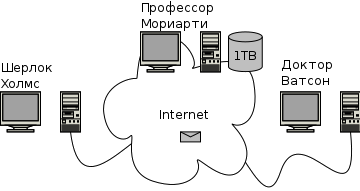
\includegraphics[width=1\textwidth]{network-3}
    \llap{
      \put(-250,100){
        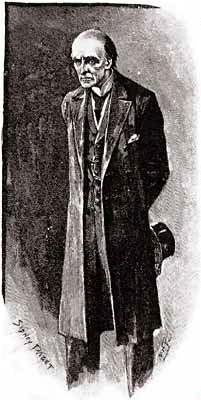
\includegraphics[height=0.4\textheight]{Pd_Moriarty_by_Sidney_Paget}
      }
    }
  \end{figure}
\end{frame}

\begin{frame}{\sc{Недостатки GnuPG -- 2.}}
  \begin{figure}[htb]
    \centering
    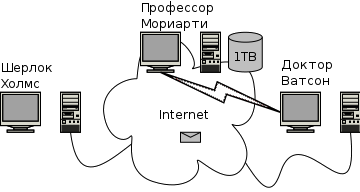
\includegraphics[width=1\textwidth]{network-4}
    \put(-120,150){
      Prof. Moriarty strikes back!
    }
    \llap{
      \put(-250,100){
        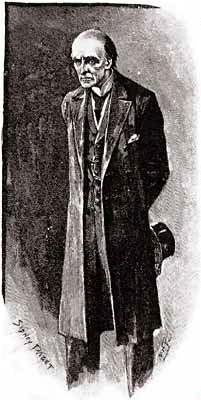
\includegraphics[height=0.4\textheight]{Pd_Moriarty_by_Sidney_Paget}
      }
    }
  \end{figure}
\end{frame}

\begin{frame}{\sc{Недостатки GnuPG -- 3.}}
  \begin{enumerate}
  \item Используются долгоживущие закрытые ключи для
    шифрования.
  \item Благодаря цифровым подписям можно с уверенностью сказать, кто
    автор сообщения, и доказать авторство третьим лицам.
  \item Относительно сложен в использовании.
  \end{enumerate}
  \bigskip
  \RaisedRightHand GnuPG не обладает свойствами, необходимыми для
обеспечения приватного разговора через IM-протокол.
\end{frame}


%%%

\section{\sc{Off-the-Record Messaging.}}

\begin{frame}{\sc{Off-the-Record Messaging.}}
  \RaisedRightHand Цель Off-the-Record Messaging (OTR) – обеспечить
  для IM свойства, присущие обычным беседам.\newline

  Возможности:
  \begin{itemize}
  \item \textbf{Шифрование} 
  \item \textbf{Аутентификация}
  \item \textbf{Отрицаемая аутентификация} (англ. \textit{deniable
      authentication}) не позволяет доказать аутентичность собеседника
    третьим лицам.
  \item \textbf{Совершенная прямая секретность} (англ. \textit{perfect
      forward secrecy}) -- компроментация долговременных ключей не
    приводит к компроментации сессионных ключей.

  \end{itemize}
  Недостатки:
  \begin{itemize}
  \item Хорошо работает только с протоколами общения в
    реальном времени.
  \end{itemize}
\end{frame}

\begin{frame}{\sc{IM-клиенты, поддерживающие OTR.}}
  \begin{columns}
    \begin{column}{0.5\textwidth}
      Из коробки:
      \begin{itemize}
      \item Adium
      \item BitlBee
      \item ChatSecure
      \item IM+
      \item Jitsi
      \item LeechCraft
      \item MCabber
      \item Psi+
      \item Xabber
      \end{itemize}
    \end{column}
    \begin{column}{0.5\textwidth}
      С использованием плагина:
      \begin{itemize}
      \item Pidgin (Gaim) -- Через плагин \texttt{pidgin-otr}
      \item Kopete
      \item Miranda IM
      \item irssi
      \item Gajim
      \item Tkabber
      \item Vacuum-IM
      \end{itemize}
    \end{column}
  \end{columns}
\end{frame}

\begin{frame}[fragile]{\sc{Установка и настройка pidgin-otr -- 1.}}
\begin{verbatim}
$ sudo apt-get install pidgin-otr
\end{verbatim}
Из меню ``Средства'' открываем список модулей и включаем OTR:
\begin{columns}
  \begin{column}{0.5\textwidth}
    \begin{figure}[htb]
      \centering
      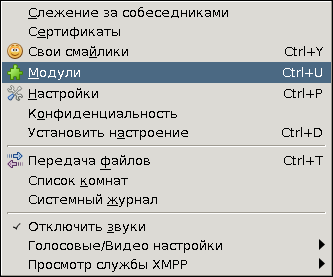
\includegraphics[clip,width=0.5\textheight]{pidgin-otr-1}
      \caption{Открытие списка модулей}
    \end{figure}
  \end{column}
  \begin{column}{0.5\textwidth}
    %% Column2
    \label{sec-3-10-2}

    \begin{figure}[htb]
      \centering
      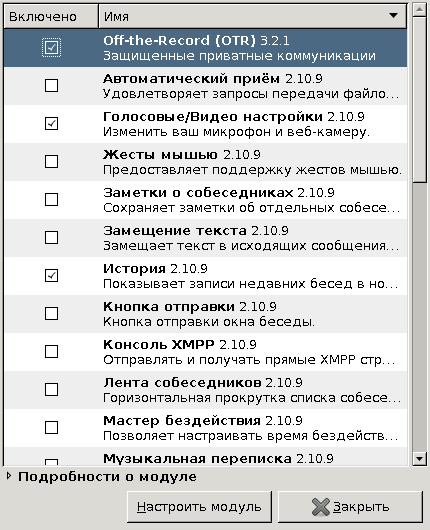
\includegraphics[clip,height=0.5\textheight]{./pidgin-otr-2}
      \caption{Включение модуля}
    \end{figure}
  \end{column}
\end{columns}
\end{frame}

\begin{frame}{\sc{Установка и настройка pidgin-otr -- 2.}}
\begin{itemize}
\item Необходимо сгенерировать ключ (нажать на кнопку ``Создать'')
    \begin{figure}[htb]
    \centering
    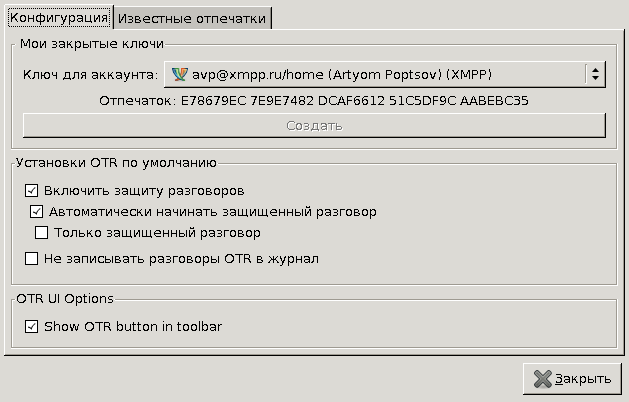
\includegraphics[clip,width=0.8\textwidth]{./pidgin-otr-3.png}
    \caption{Генерация закрытого ключа}
    \end{figure}
\end{itemize}
\end{frame}

\begin{frame}{\sc{Установка и настройка pidgin-otr -- 3.}}
Далее следует аутентифицировать собеседника при первом разговоре:
\begin{columns}
\begin{column}{0.5\textwidth}
  \begin{figure}[htb]
    \centering
    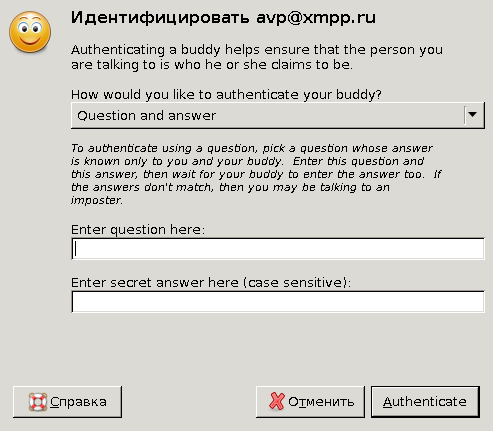
\includegraphics[clip,width=0.5\textheight]{./pidgin-otr-4}
    \caption{Аутентификация с помощью вопроса}
  \end{figure}
\end{column}
\begin{column}{0.5\textwidth}
  \begin{figure}[htb]
    \centering
    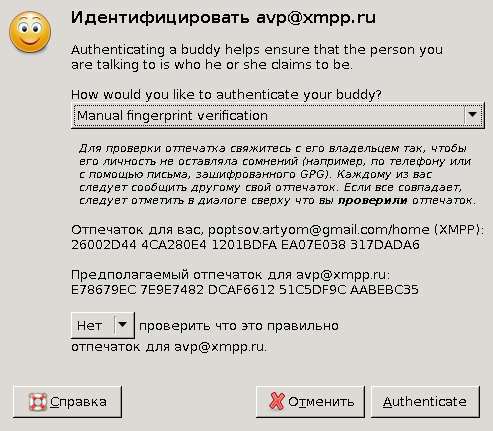
\includegraphics[clip,width=0.5\textheight]{./pidgin-otr-5}
    \caption{Аутентификация по отпечатку ключа}
  \end{figure}
\end{column}
\end{columns}
\end{frame}


%%%

\subsection{Спасибо за внимание!}

\begin{frame}{\sc{Спасибо за внимание!}}
  \large

  Контакты:
  \begin{itemize}
  \item Web-сайт: poptsov-artyom.narod.ru
  \item Эл. почта: \url{poptsov.artyom@gmail.com}
  \item Отпечаток ключа GnuPG: D0C2 EAC1 3310 822D 98DE  B57C E9C5 A2D9 0898 A02F
  \end{itemize}
  \medskip

  Презентация и её ``исходники'' под лицензией Creative Commons:
  \url{github.com/artyom-poptsov/talks/tree/master/defcon-nn/} \\[10pt]

  \bigskip

  \huge Вопросы?
\end{frame}

\begin{frame}{\sc{Лицензия.}}
  Copyright \textcopyright 2017 Artyom V. Poptsov
  <poptsov.artyom@gmail.com> \newline

  Права на копирование других изображений, использованных в данной
  работе, принадлежат их владельцам. \newline

  Данная работа распространяется на условиях лицензии Creative Commons
  Attribution-ShareAlike 4.0 International:
  \url{https://creativecommons.org/licenses/by-sa/4.0/}
\end{frame}

\begin{frame}{\sc{Использованные материалы.}}
  Использованные источники:
  \begin{itemize}
  \item Ian Goldberg, ``OTR messaging'' (CC-BY-NC-ND 3.0) --
    \url{https://archive.org/details/IanGoldberg-OtrMessaging}
  \item Nikita Borisov, Ian Goldberg, Eric Brewer
    (2004-10-28). ``Off-the-Record Communication, or, Why Not To Use
    PGP'': \url{https://otr.cypherpunks.ca/otr-wpes.pdf}
  \item Ian Goldberg, ``Off-the-Record Messaging: Useful Security and
    Privacy for IM'': \url{https://www.youtube.com/watch?v=uI1x-z5oafc}
  \end{itemize}
  Основа для дизайна:
  \begin{itemize}
  \item Richardson, Milton Thomas (ed.), ``Practical blacksmithing'',
    volume 1 (PD) --
    \url{https://archive.org/details/practicalblacksm01richuoft}
  \item Richardson, Milton Thomas (ed.), ``Practical blacksmithing'',
    volume 2 (PD) --
    \url{https://archive.org/details/practicalblacksm00rich}
  \end{itemize}
\end{frame}


%%%

\end{document}

%%% 0x01.tex ends here
